 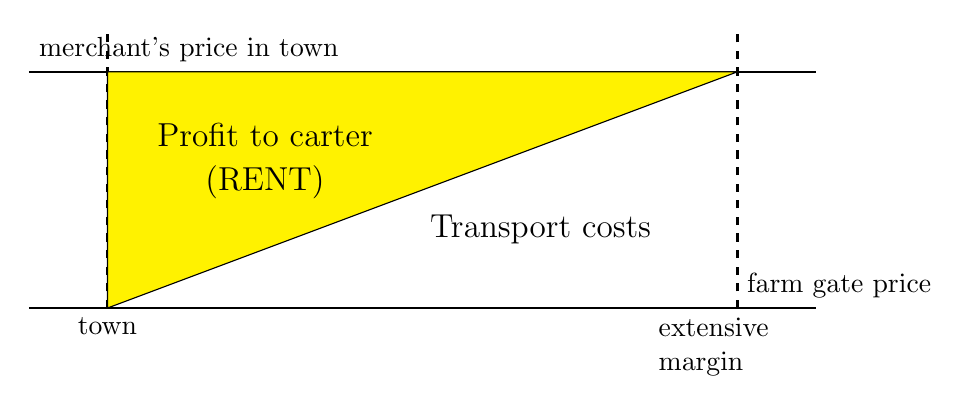
\begin{tikzpicture}[domain=0:2]
%\draw[thick,color=gray,step=.5cm, dashed] (-0.5,-.5) grid (3,3);
%\draw[line width=.01, green ] (0,0) -- (10,0) node[right  ] {Distance};
\node at (1,0) [below] {town};
\draw[thick ] (0,3)node[above right] {merchant's price in town} -- (10,3) ;
\draw[thick ] (0,0)  -- (10,0); 

draw[thick,color=red] (1.5,0) -- (1.5,1) node[below right] {Fixed cost} -- (1.5,1.5) --(10,3.25)node[above left] {total cost};
\draw[thick, dashed ] (1,0) -- (1,3.5) ;
\draw[thick, dashed ] (9,0)node[below,text width=2cm] {extensive margin} -- (9,3.5) ;
%\draw[ultra thick, blue,<-> ] (3,1.8) -- (3,2.5)node[left] {annual rent at a} -- (3,3) ; 
\draw[fill=yellow] (1,0) --(9,3)--(1,3) --cycle;
\node at (9,0)[above right] {farm gate price};
\node  at (6.5,1){\large Transport costs};
\node  at (3.,2.2){\large Profit to carter};
\node  at (3.,1.6){\large (RENT)};
\end{tikzpicture} 